\section{Contraintes}
Réalisation d'un effet \emph{fisheye} en flex. L'idée est d'appliquer l'effet sur les conteneur présents dans le conteneur appliquant le layout \emph{fisheye}, sous la forme d'une grille dont les éléments grandisse en fonction de la proximité avec la souris.

Dans l'idéal, l'effet produit doit minimiser l'espace entre les conteneurs.

\section{Analyse \& implémentation}

Nous avons fait le choix de créer un layout \emph{fisheye} assurant les traitements nécessaire à la réalisation de l'effet. Pour cela, nous avons utilisé le namespace \emph{spark} permettant de dissocier le container du layout. Il sera ainsi possible d'associer le layout personnalisé à n'importe quel container spark. Le layout appliquera l'effet sur tous les containers dont le container parent est celui sur lequel est appliqué le layout \emph{fisheye}.

Pour la réalisation de ce layout, nous avons eu trois approches qui seront détaillées ci-après.

\subsection{Approche globale}
\label{subsec:globale}
Cette approche suppose qu'il est possible, en connaissant la position de la souris et la position d'un bloc, de le placer et le dimensionner exactement sur la grille. Les caractéristiques du bloc ne dépendent donc pas du placement des autres blocs voisins.

Le layout peut être paramétré de la manière suivante :

\begin{description}
  \item[maxSize] Taille maximum de l'élément dans la grille,
  \item[minSize] Taille minimum de l'élément dans la grille,
  \item[spread] Propagation de l'agrandissement autour de la souris,
\end{description}

Ainsi le layout va initialiser les éléments sur une grille de la manière suivante :
\begin{figure}[H]
  \centering
  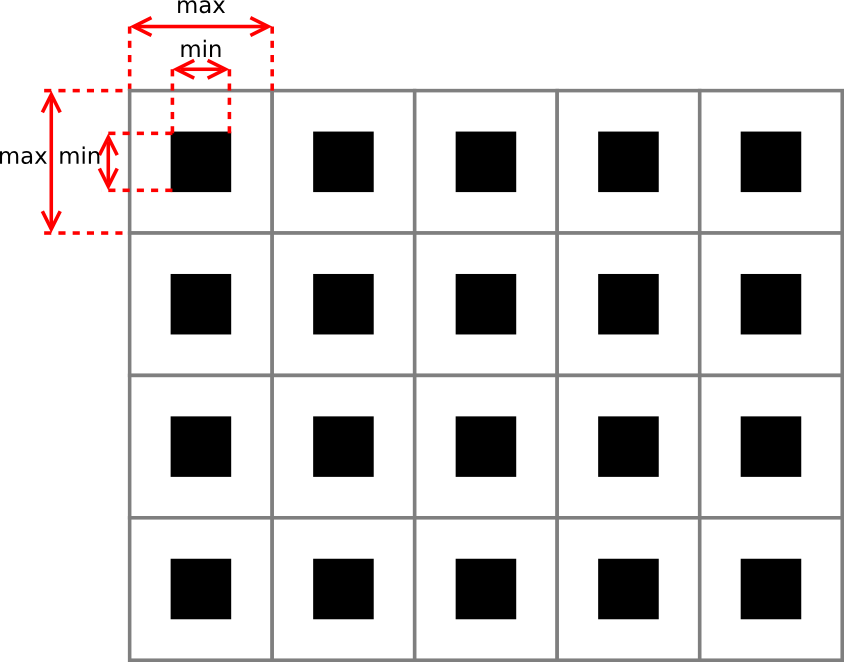
\includegraphics[width=.7\textwidth]{../resources/illustrations/grob_app_init}
  \caption{Initialisation des éléments avec l'approche globale.}
\end{figure}

Un \emph{eventlistener} capture les mouvements de la souris dans le but de mettre à jour chaque \emph{container} de la grille.

\begin{figure}[H]
  \centering
  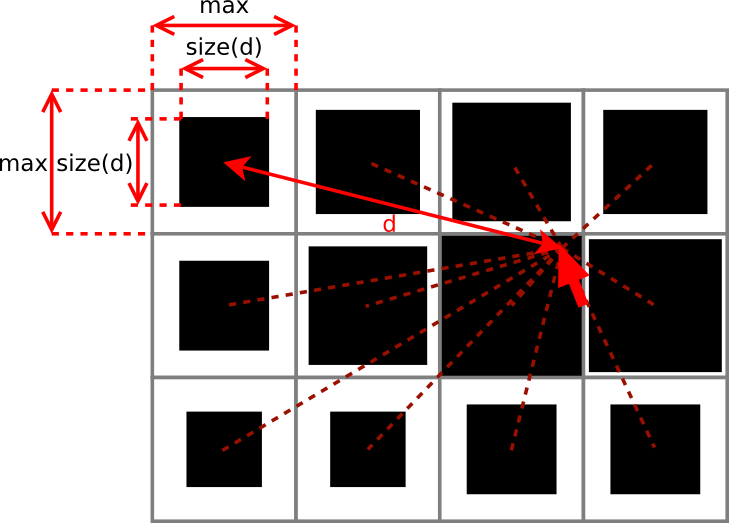
\includegraphics[width=.7\textwidth]{../resources/illustrations/grob_app_mouse}
  \caption{Mise à jours des éléments avec l'approche globale.}
\end{figure}

La taille des éléments sont mis à jours en fonction de la distance entre le centre du block et le pointeur de la souris. Dans tous les cas les éléments restent alignés dans la grille par le fait que les centres des objets ne sont pas déplacés.

Après implémentation et test avec des containers colorés en noir, on obtient ceci :

\begin{figure}[H]
  \centering
  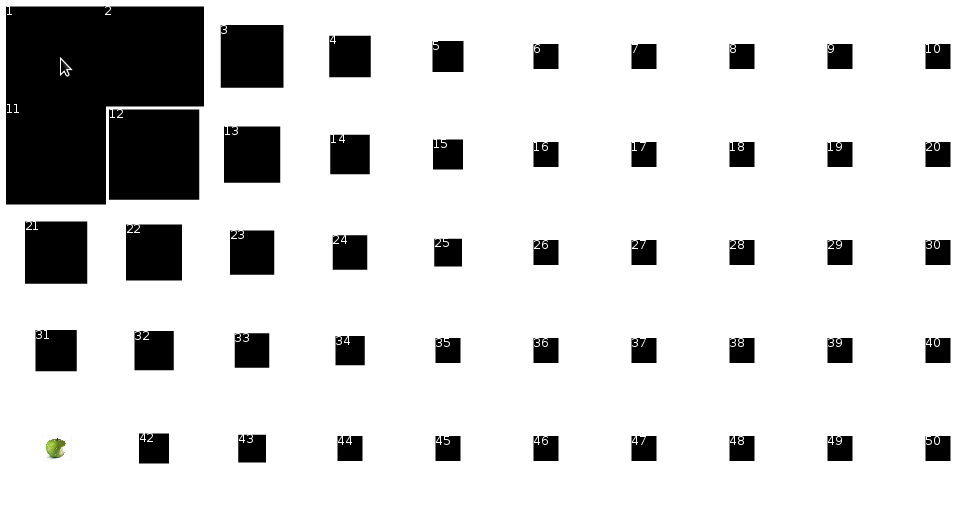
\includegraphics[width=.7\textwidth]{../resources/illustrations/c1}
  \caption{Premier aperçu.}
\end{figure}

\begin{figure}[H]
  \centering
  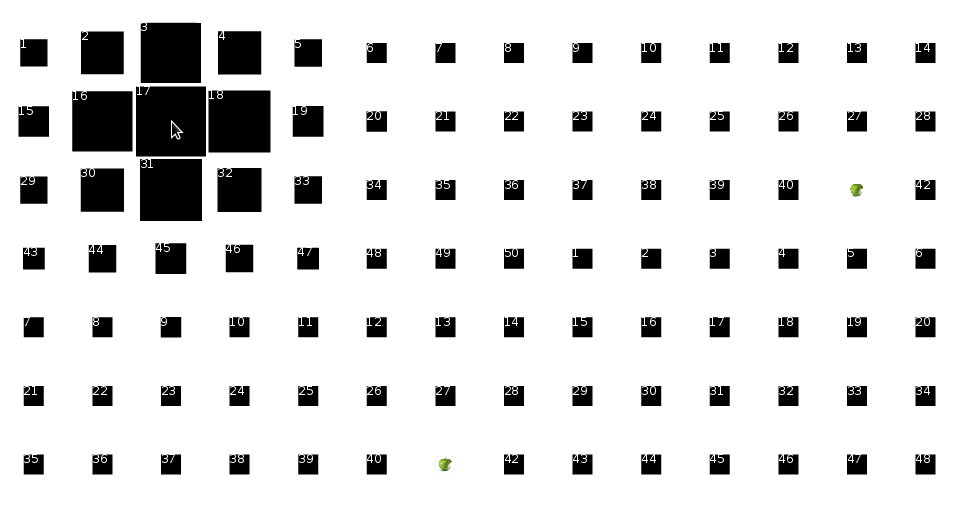
\includegraphics[width=.7\textwidth]{../resources/illustrations/c2}
  \caption{Second aperçu.}
\end{figure}

L'avantage de ce type d'approche est d'arriver rapidement à un résultat fluide et  satisfaisant. Le principal problème réside dans l'espacement entre les éléments de la grille. Un solution\footnote{Solution non implémentée.} pourrait consister en la mise en place d'une attraction des éléments vers le pointeur de la souris : plus les éléments sont éloignés, plus ils sont attirés vers la souris. On obtiendrait quelque chose comme suit :

\begin{figure}[H]
  \centering
  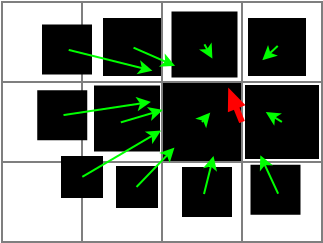
\includegraphics[width=.7\textwidth]{../resources/illustrations/grob_app_evo}
  \caption{Évolution permettant de réduire l'espace entre les éléments de la grille.}
\end{figure}

\subsection{Approche propagée}
\label{subsec:propage}

Cette approche est différente. Les dimensions et la position de chaque élément dépend des autre, et sont affectés au travers d'un parcours séquentiel.

Ici les éléments sont initialisé par une valeur moyenne ainsi qu'une marge entre les éléments.

\begin{figure}[H]
  \centering
  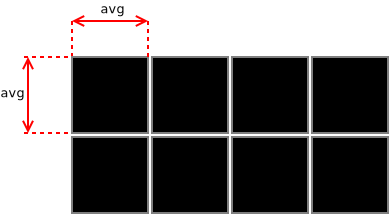
\includegraphics[width=.7\textwidth]{../resources/illustrations/seq_app_init}
  \caption{Initialisation par la méthode propagée.}
\end{figure}

Lors d'un mouvement de souris, le parcours débute par l'élément le plus proche de la souris, affecte les positions et tailles des éléments sur la ligne, puis le traitement est effectué de manière récursive pour chaque autre ligne.

\begin{figure}[H]
  \centering
  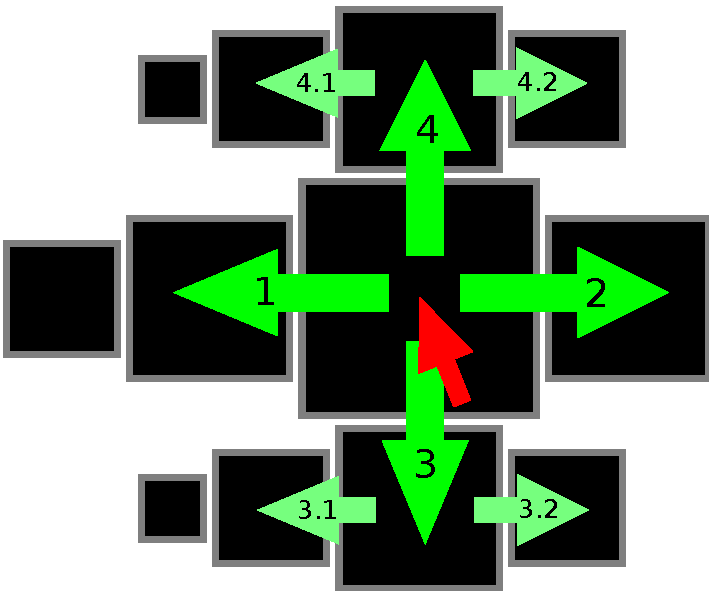
\includegraphics[width=.7\textwidth]{../resources/illustrations/seq_app_mouse}
  \caption{Évolution permettant de réduire l'espace entre les éléments de la grille.}
\end{figure}

Ce rendu a été réalisé mais n'est pas exploitable pour deux raisons :

\begin{itemize}
  \item pas de fluidité lors du passage de la souris entre deux éléments,
  \item disposition peu ergonomique.
\end{itemize}

Dans le but d'améliorer le second point, la disposition des éléments des ligne pourrait être améliorer\footnote{Amélioration non implémentée.}. La première évolution propose de contraindre la distribution des éléments de chaque ligne en se basant sur la grille générée au fur et à mesure du parcours. La seconde évolution fonctionne de la même manière, mais déplace les éléments dans le coin le plus proche de l'élément sélectionné.

\begin{minipage}[H]{.5\linewidth}
\begin{figure}[H]
  \centering
  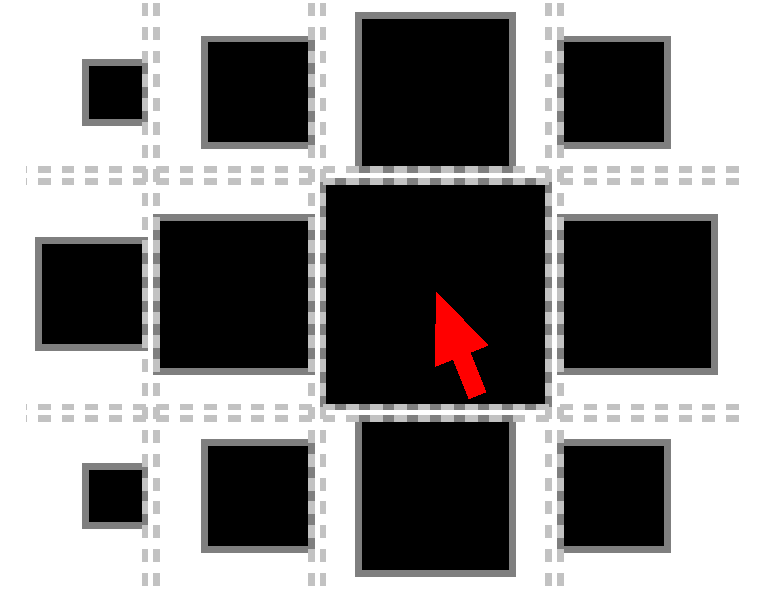
\includegraphics[width=\textwidth]{../resources/illustrations/seq_app_mouse_v2}
  \caption{Première évolution permettant un meilleur affichage de la grille.}
\end{figure}
\end{minipage}
\begin{minipage}[H]{.5\linewidth}
\begin{figure}[H]
  \centering
  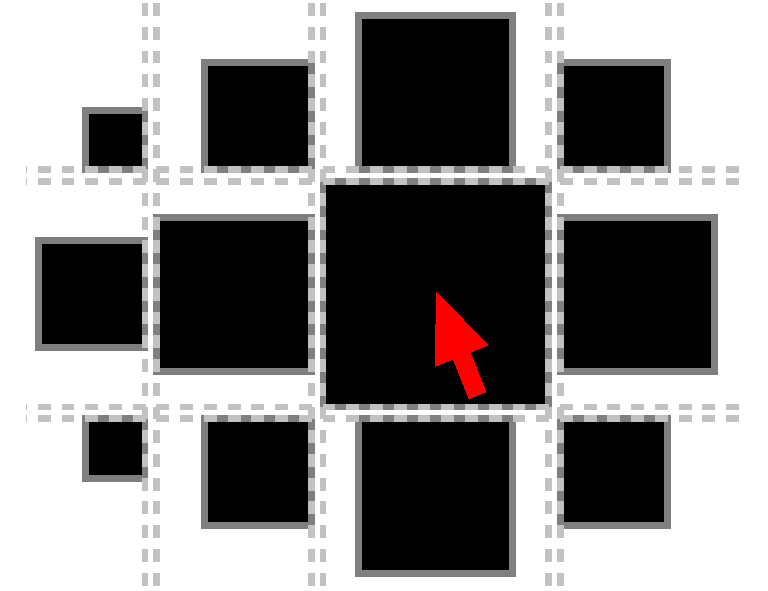
\includegraphics[width=\textwidth]{../resources/illustrations/seq_app_mouse_v3}
  \caption{Seconde évolution permettant un meilleur affichage de la grille.}
\end{figure}
\end{minipage}

\subsection{Approche avancée}

La dernière approche est une approche avancée axée sur l'aspect mathématique du problème, dans le but de réaliser un \og vrai \fg{} effet \emph{fisheye}. L'idée est de considérer l'ensemble des éléments comme un tableau d'éléments puis de jouer sur la largeur des colonnes et la hauteur des lignes.

\begin{figure}[H]
  \centering
  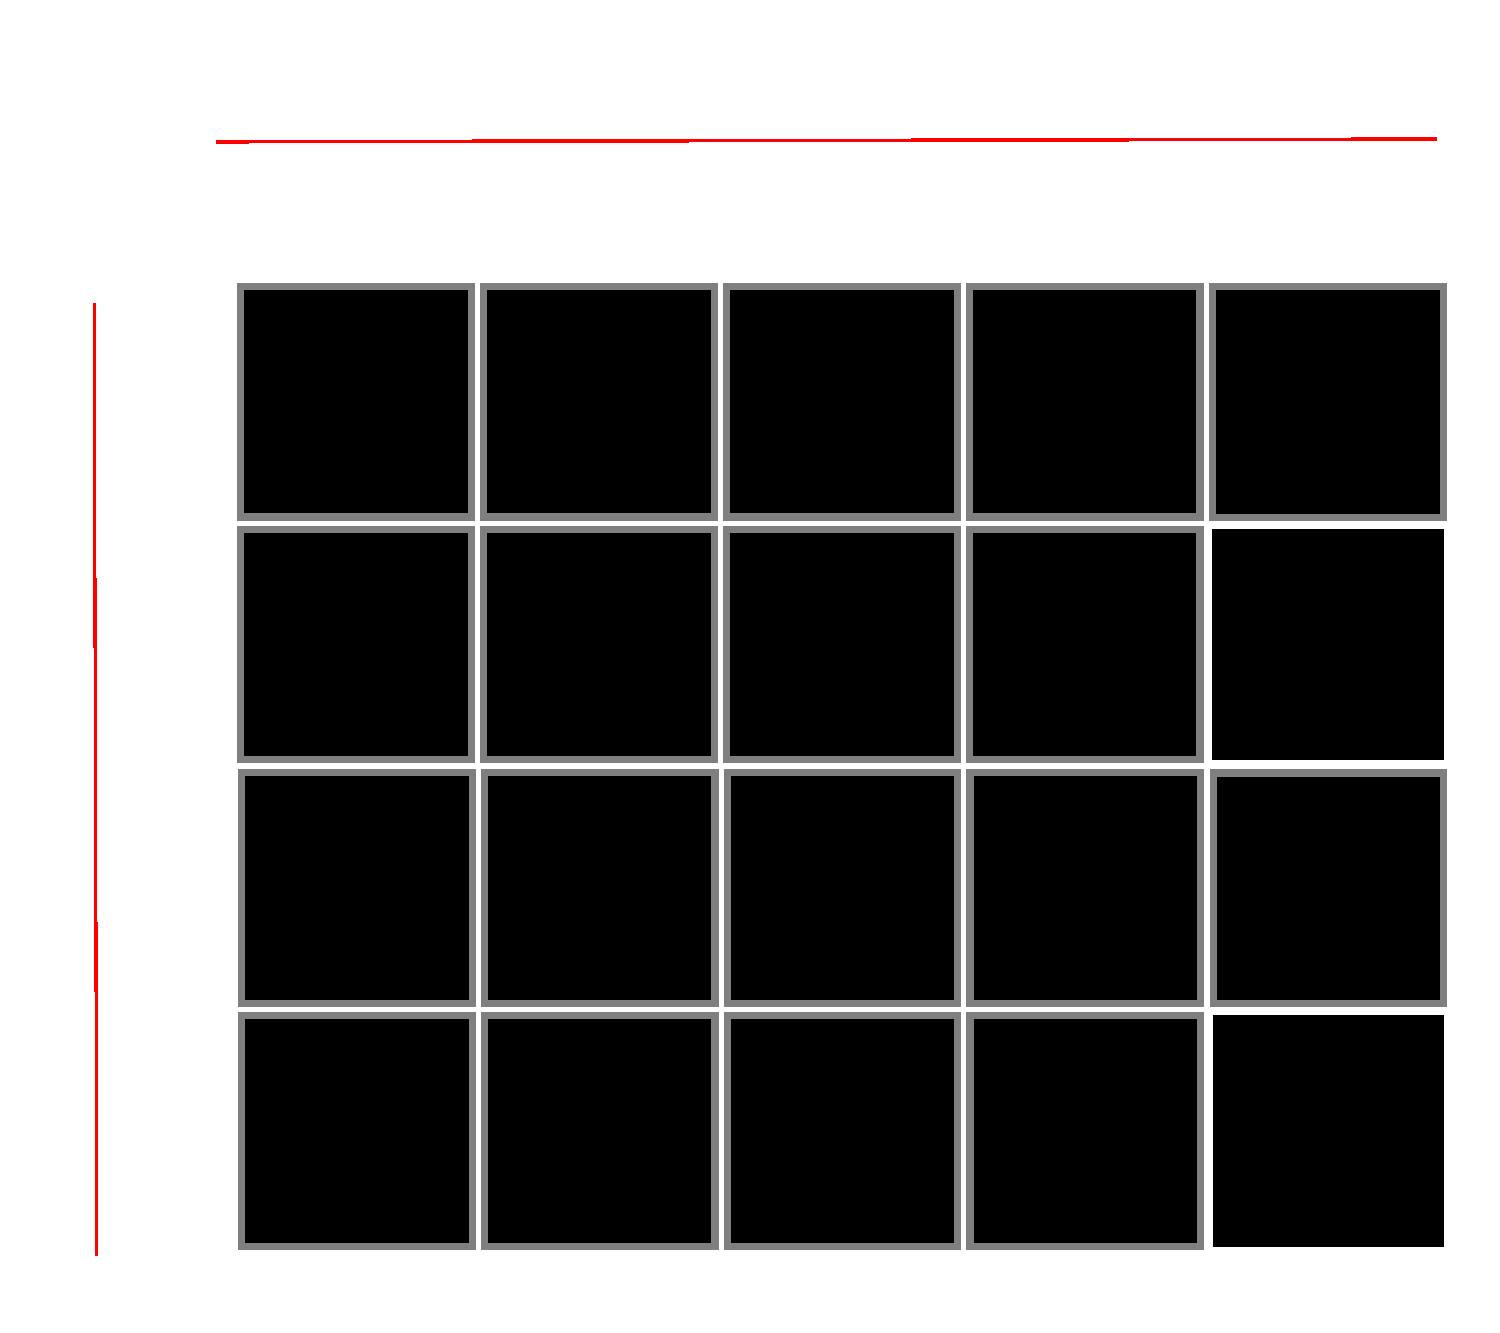
\includegraphics[width=0.7\textwidth]{../resources/illustrations/js_1}
  \caption{Grille d'éléments sans présence de la souris}
  \label{fig:js_1}
\end{figure}

La figure \ref{fig:js_1} ci-dessus représente l'état du tableau en
l'absence de la souris. Dans ce cas, la largeur et la hauteur des
cellules sont représentés par une fonction constante. La figure
\ref{fig:js_2} montre comment la largeur et la hauteur des cellules
sont modifiées par la présence de la souris. La nouvelle taille des
cellules est calculée grâce à deux fonctions gaussiennes indépendante,
une pour la largeur et une autre pour la hauteur.  

\begin{figure}[H]
  \centering
  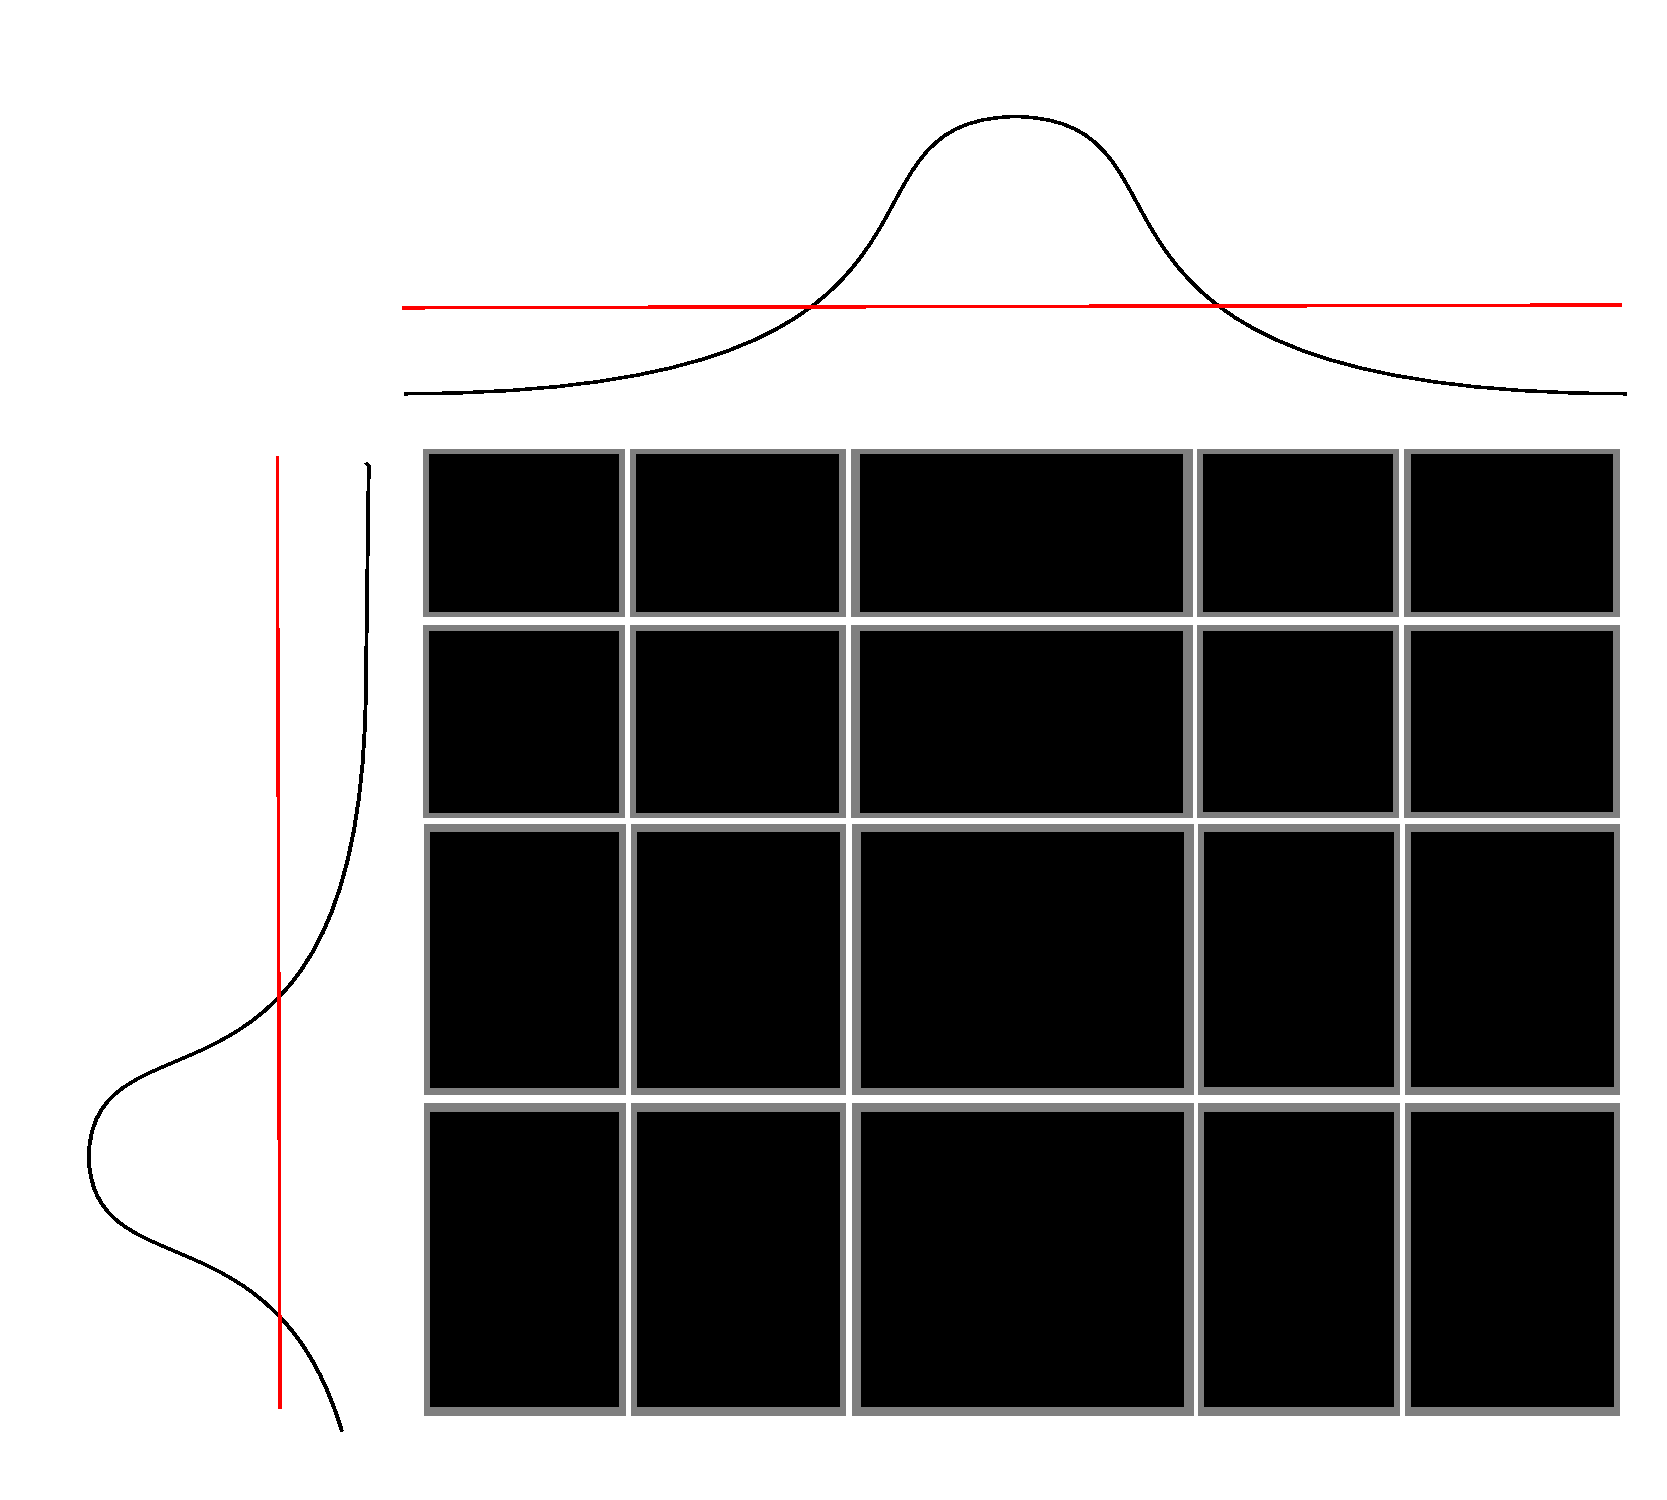
\includegraphics[width=0.7\textwidth]{../resources/illustrations/js_2}
  \caption{Grille d'éléments modifié par la présence de la souris}
    \label{fig:js_2}
\end{figure}

Ces fonctions sont 
\begin{equation}
taille\_par\_defaut + \frac{facteur\_grossissement}{(dist/attenuation)^{2}+0.5}-facteur\_grossissement
\end{equation}

\begin{figure}[H]
  \centering
  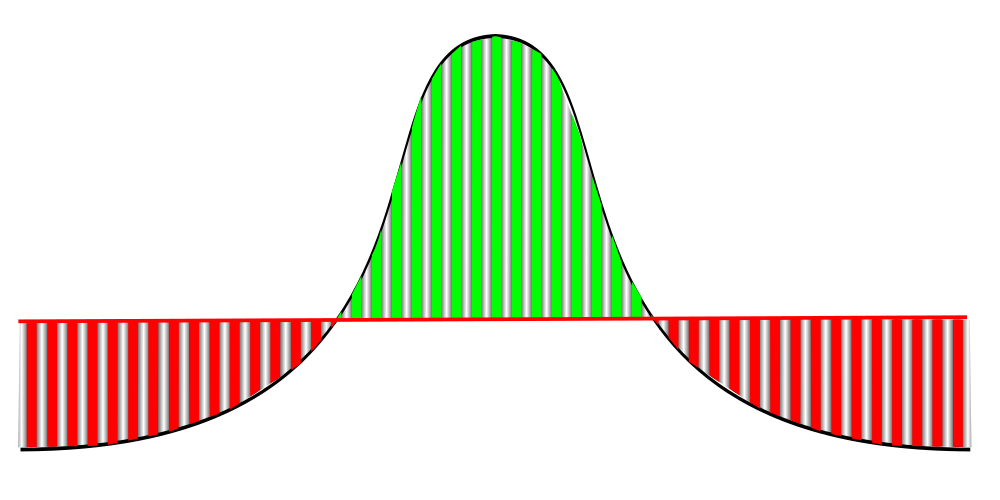
\includegraphics[width=0.7\textwidth]{../resources/illustrations/js_3}
  \caption{Courbe de déformation}
    \label{fig:js_3}
\end{figure}

La surface verte représente le gain de taille par rapport à la taille par défaut, la surface rouge représente la perte de taille. L'enjeu lors du parcours de la souris est de faire en sorte que ces deux surface soient égales.

Ce problème est mis en évidence dans le pire des cas lorsque la souris est au maximum contre un bord. Comme il est possible de le voir sur la figure~\ref{fig:js_4}, dans ce cas la surface de gain est bien plus élevé que la surface de perte. Dans le but d'atteindre une répartition parfaite entre ces deux surface, la différence entre la surface rouge est la surface verte est calculé, puis   redistribuée sur tous les éléments de la ligne et/ou colonne. La figure~\ref{fig:js_5} représente le résultat obtenu.

\begin{minipage}[H]{.5\textwidth}
\begin{figure}[H]
  \centering
  \vspace{.4cm}
  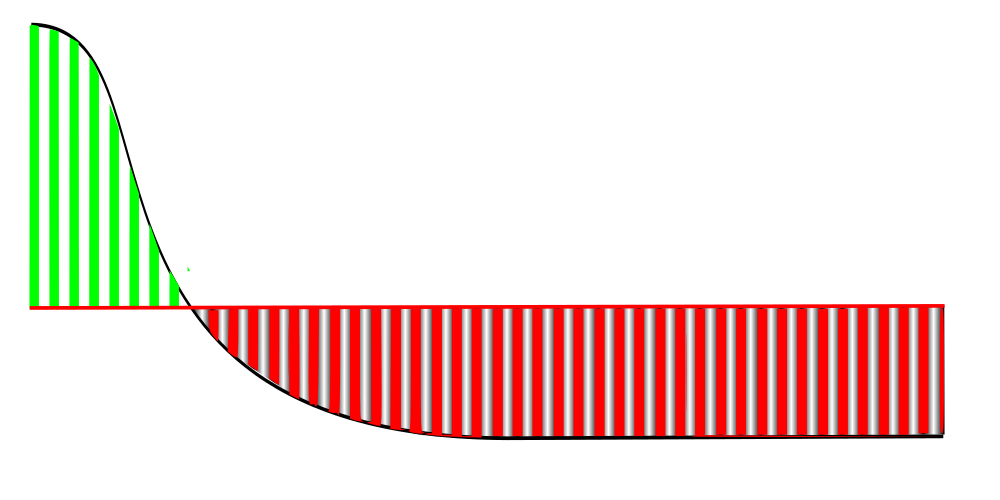
\includegraphics[width=\textwidth]{../resources/illustrations/js_4}
  \caption{Courbe de déformation}
    \label{fig:js_4}
\end{figure}
\end{minipage}
\begin{minipage}[H]{.5\textwidth}
\begin{figure}[H]
  \centering
  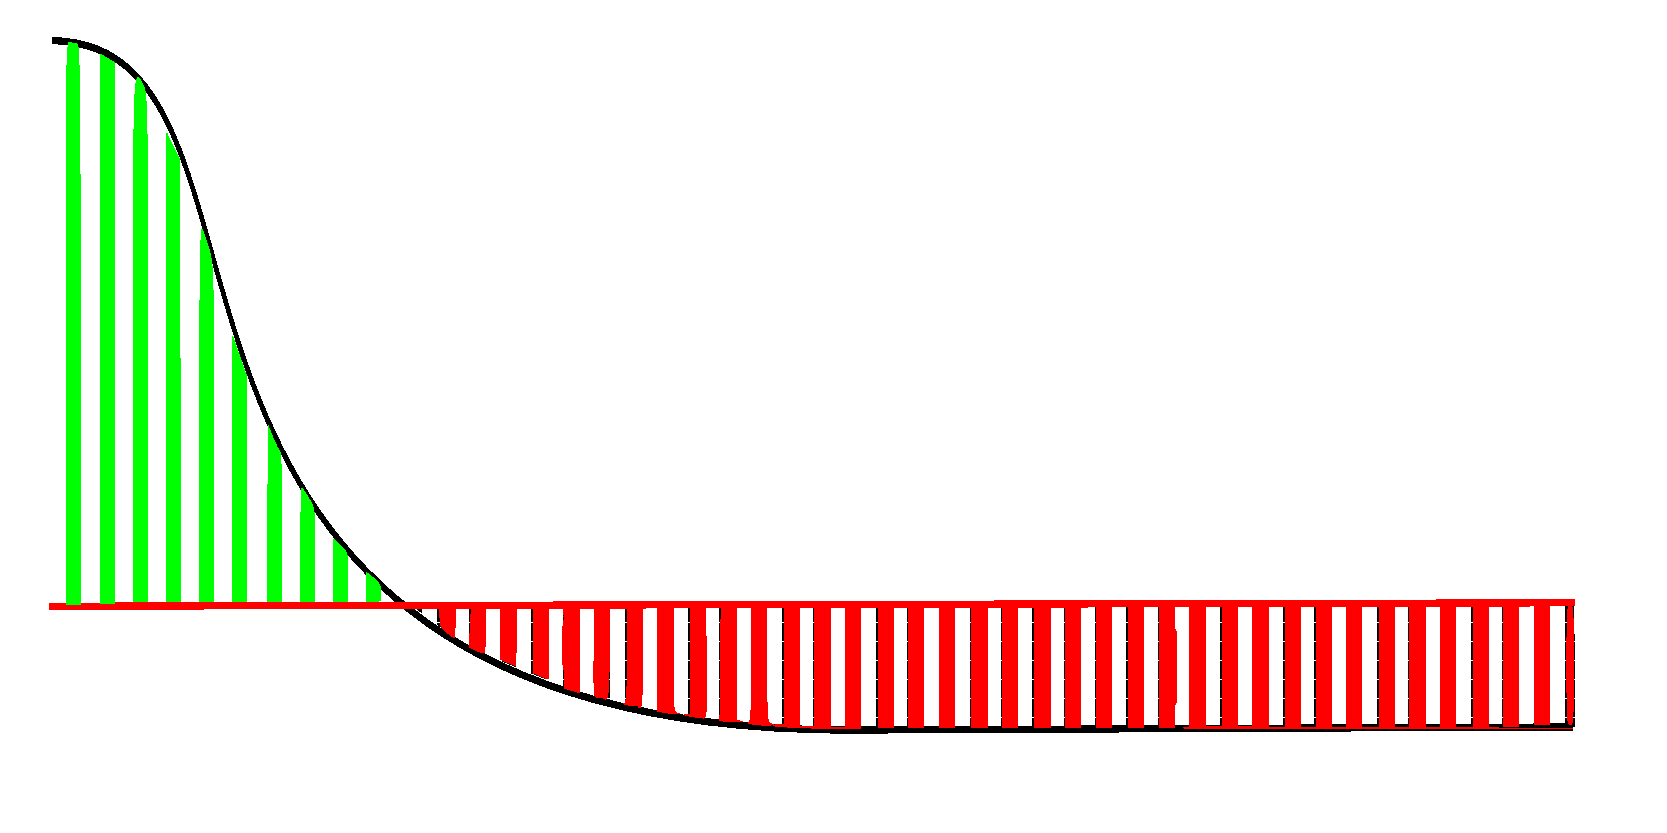
\includegraphics[width=\textwidth]{../resources/illustrations/js_5}
  \vspace{.05cm}
  \caption{Courbe de déformation}
  \label{fig:js_5}
\end{figure}
\end{minipage}

\subsubsection{Implémentation JavaScript}

Un premier prototype a été réalisé en javascript / HTML5, avec deux \emph{sliders} permettant la modification à la volé de facteur de grossissement, et de l'atténuation. Un \emph{checkbox} permet également la représentation des élément sous la forme de carrés.

\begin{figure}[H]
  \centering
  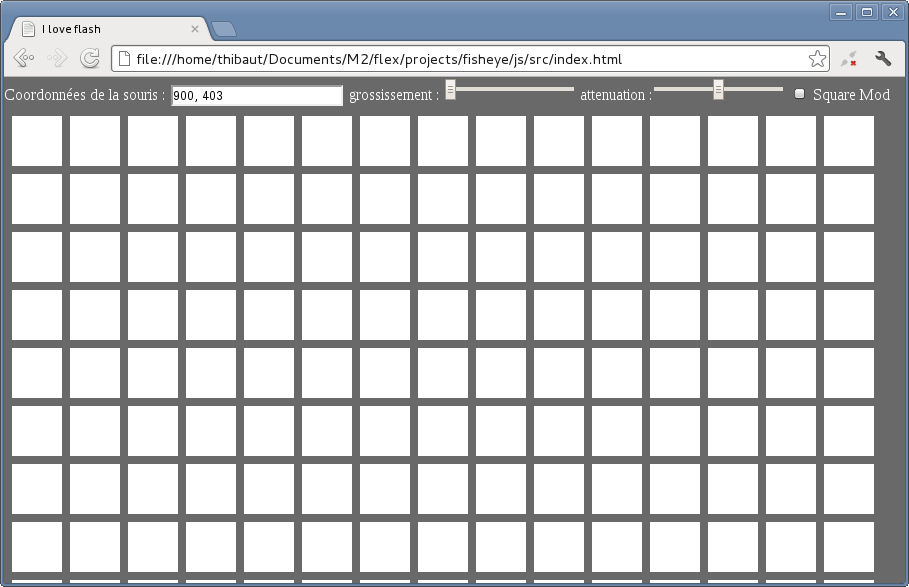
\includegraphics[width=\textwidth]{../resources/illustrations/js_screen_1}
  \caption{Aperçu de l'effet fisheye JS sans facteur de grossissement (grille de base).}
  \label{fig:js_6}
\end{figure}
\begin{minipage}[H]{.5\textwidth}
\begin{figure}[H]
  \centering
  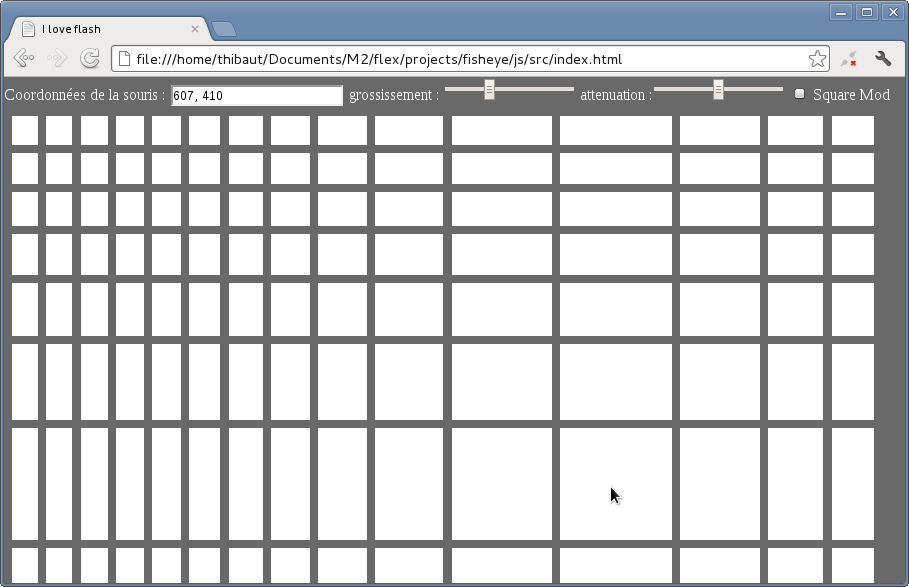
\includegraphics[width=\textwidth]{../resources/illustrations/js_screen_2}
  \caption{Aperçu de l'effet fisheye JS avec facteur de grossissement.}
  \label{fig:js_6}
\end{figure}
\end{minipage}
\begin{minipage}[H]{.5\textwidth}
\begin{figure}[H]
  \centering
  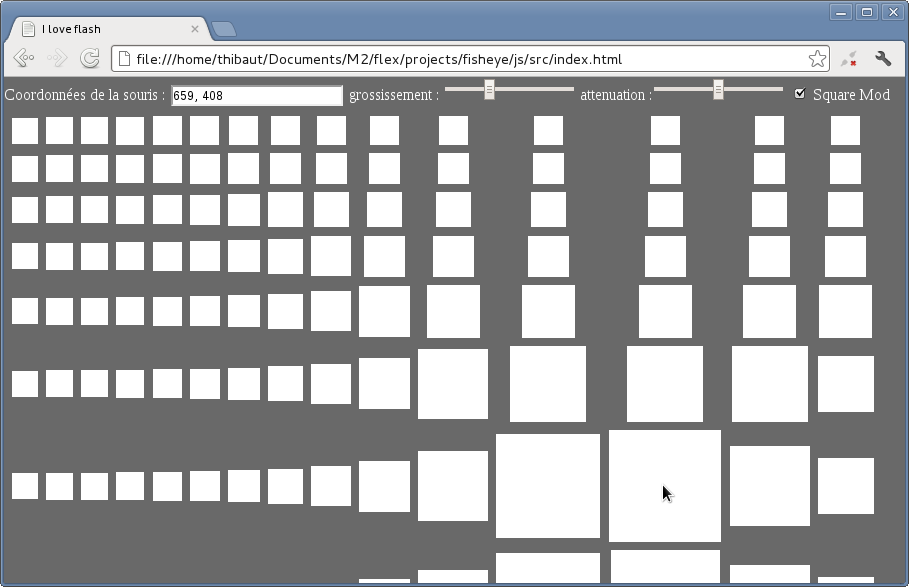
\includegraphics[width=\textwidth]{../resources/illustrations/js_screen_3}
  \caption{Aperçu de l'effet fisheye JS avec facteur de grossissement (mode carré).}
  \label{fig:js_6}
\end{figure}
\end{minipage}

\subsubsection{Implémentation Flex}

Un prototype reposant sur les mêmes algorithmes à été développé en flex. Il implémente les même fonctionnalités que son homologues JavaScript, et est basé sur l'implémentation d'un \emph{Layout Spark} personnalisé, comme les version vues dans les sections~\ref{subsec:globale} et~\ref{subsec:propage}.

\begin{figure}[H]
  \centering
  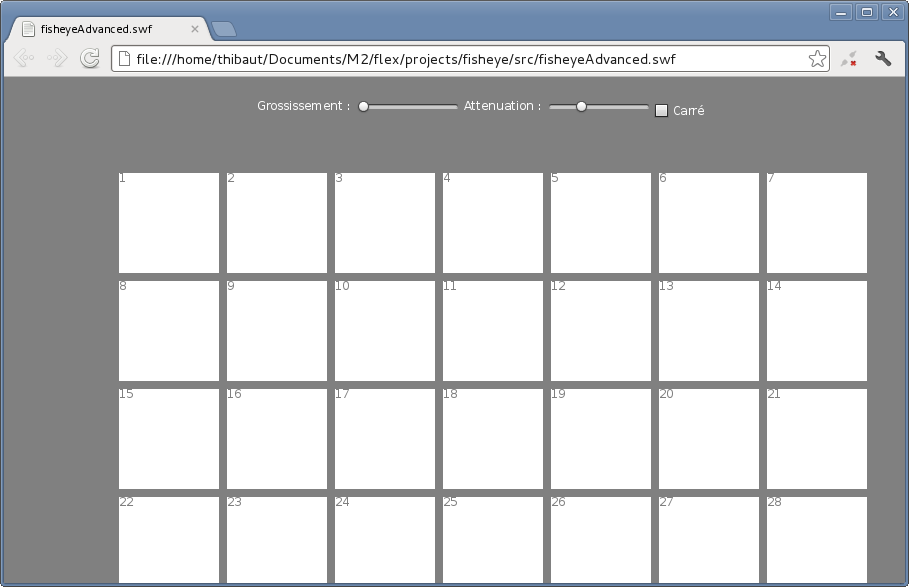
\includegraphics[width=\textwidth]{../resources/illustrations/flex_screen_1}
  \caption{Aperçu de l'effet fisheye Flex sans facteur de grossissement (grille de base).}
  \label{fig:js_6}
\end{figure}
\begin{minipage}[H]{.5\textwidth}
\begin{figure}[H]
  \centering
  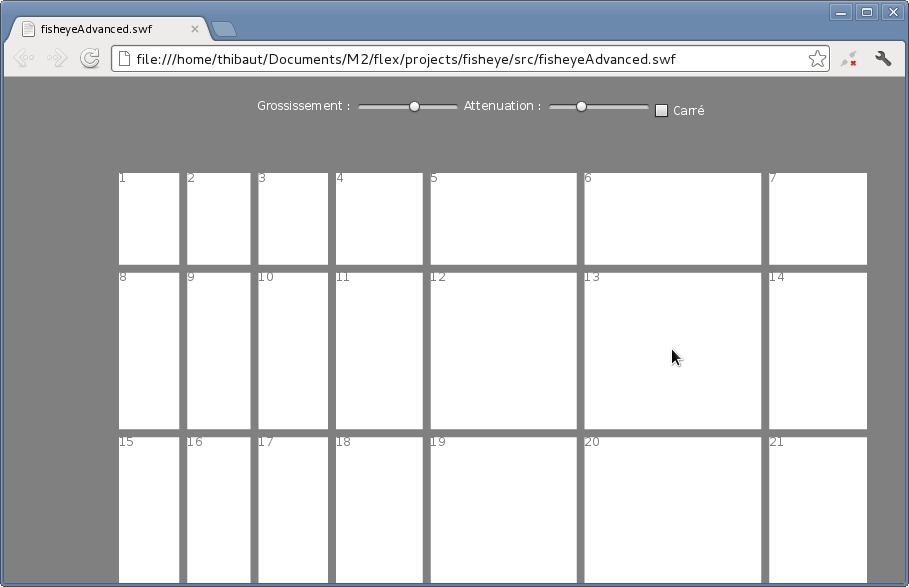
\includegraphics[width=\textwidth]{../resources/illustrations/flex_screen_2}
  \caption{Aperçu de l'effet fisheye Flex avec facteur de grossissement.}
  \label{fig:js_6}
\end{figure}
\end{minipage}
\begin{minipage}[H]{.5\textwidth}
\begin{figure}[H]
  \centering
  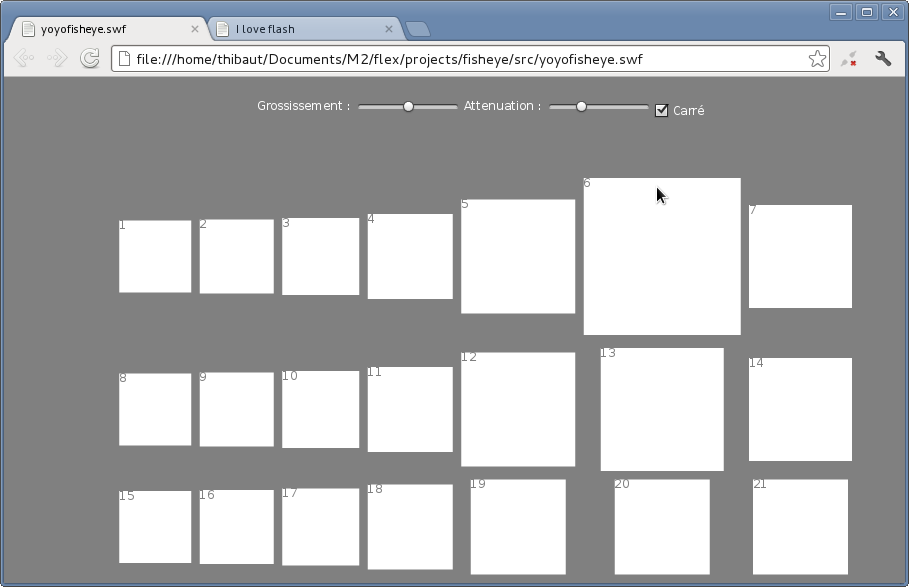
\includegraphics[width=\textwidth]{../resources/illustrations/flex_screen_3}
  \caption{Aperçu de l'effet fisheye Flex avec facteur de grossissement (mode carré).}
  \label{fig:js_6}
\end{figure}
\end{minipage}

\section{Environnement de travail}

Dans le but de réellement découvrir flex, nous avons fait le choix de ne pas utiliser Flash Builder. Le développement a donc été effectué sous GNU/Linux à l'aide d'un éditeur de texte avec complétion syntaxique pour \emph{mxml} et les classes \emph{actionscript}. La compilation a été exécutée en ligne de commande avec les compilateur \emph{mxmlc}.

Aucune version d'Air n'étant disponible sous GNU/Linux, nous avons testé nos applications avec le FlashPlugin, en lançant les fichiers \emph{swf} avec un navigateur.

\section{README}

Les sources de ce projet sont disponibles sur notre dépôt GIT (Github) à l'adresse suivante :
\begin{center}
  \href{https://github.com/fishfinger/fisheyelayout}{\texttt{https://github.com/fishfinger/fisheyelayout}}
\end{center}

\begin{description}
  \item[Fichiers compilés] disponibles dans le dossier \texttt{swf} à la racine.
  \item[Sources] disponibles dans le dossier \texttt{src} ) à la racine. Les différents \emph{Layout} sont disponibles dans le \emph{package} \texttt{custom.layouts}.
  \item[Documents] disponibles dans le dossier \texttt{docs}. Y sont présents la présentation et le présent rapport.
\end{description}